\documentclass{article}
\usepackage{graphicx}
\usepackage{amsmath}
\usepackage{float}
\usepackage{amsfonts}
\usepackage{listings}
\usepackage{xcolor}
\usepackage[utf8]{inputenc}
\usepackage{hyperref}
\usepackage{fancybox}
\usepackage{booktabs}
\usepackage{array}
\usepackage{tikz}
\usepackage{amsfonts}
\usepackage{dsfont}
\usepackage{pgfplots}
\pgfplotsset{compat=1.18}
\usepackage[margin=2cm]{geometry}
\usepackage[french]{babel} % Pour les éléments en français
\usetikzlibrary{shapes, arrows.meta, positioning}
\usepackage[labelfont=bf, font=small]{caption}  % Pour personnaliser le titre de la figure


\title{TP2 ADM Classification automatique}
\author{SCAIA Matteo et MARIAC Damien}
\date{\today} 

\begin{document}

\maketitle

\begin{figure}[h] 
    \centering
    
\includegraphics[width=0.5\textwidth]{ssd_logo.png} 
\end{figure}

\begin{figure}[h] 
    \centering
    
\includegraphics[width=0.5\textwidth]{logo_um_2022_rouge_RVB.png} 
\end{figure}

\newpage

\tableofcontents

\newpage
\section{Treillis de Galois}
\subsection{Introduction}
Le treillis de Galois est une structure mathématique utilisée en analyse de données pour extraire des règles d’implication. Il est construit à partir de données décrites par des propriétés booléennes, permettant de représenter les relations entre ces propriétés et les ensembles d’objets associés. 
Le treillis de Galois peut également intégrer des relations liant les données entre elles.
\subsection{Interprétation et création du treillis de Galois}
Dans cette question, nous allons analyser le treillis de Galois construit à partir des données fournies par le sujet afin de modéliser les relations entre les films et leurs caractéristiques.
\begin{figure}[h]
    \centering
    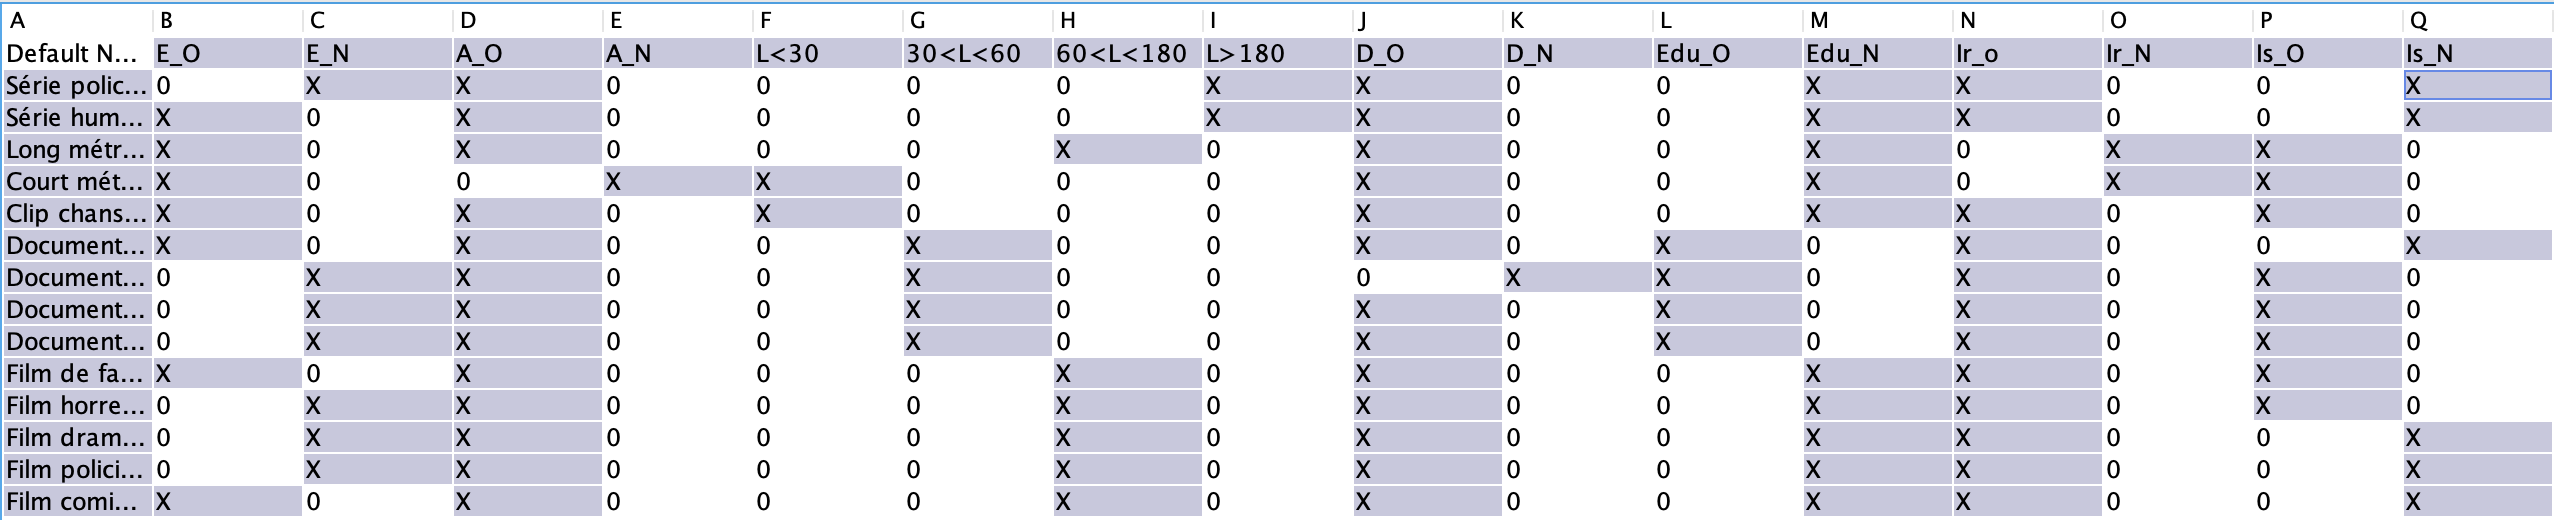
\includegraphics[width=0.7\textwidth]{tableau.png}
    \caption{Tableau des relations binaires}
    \label{fig:tableau} 
\end{figure}
\\
À l'aide du logiciel Galicia, nous obtenons le treillis de Galois suivant :
\begin{figure}[h]
    \centering
    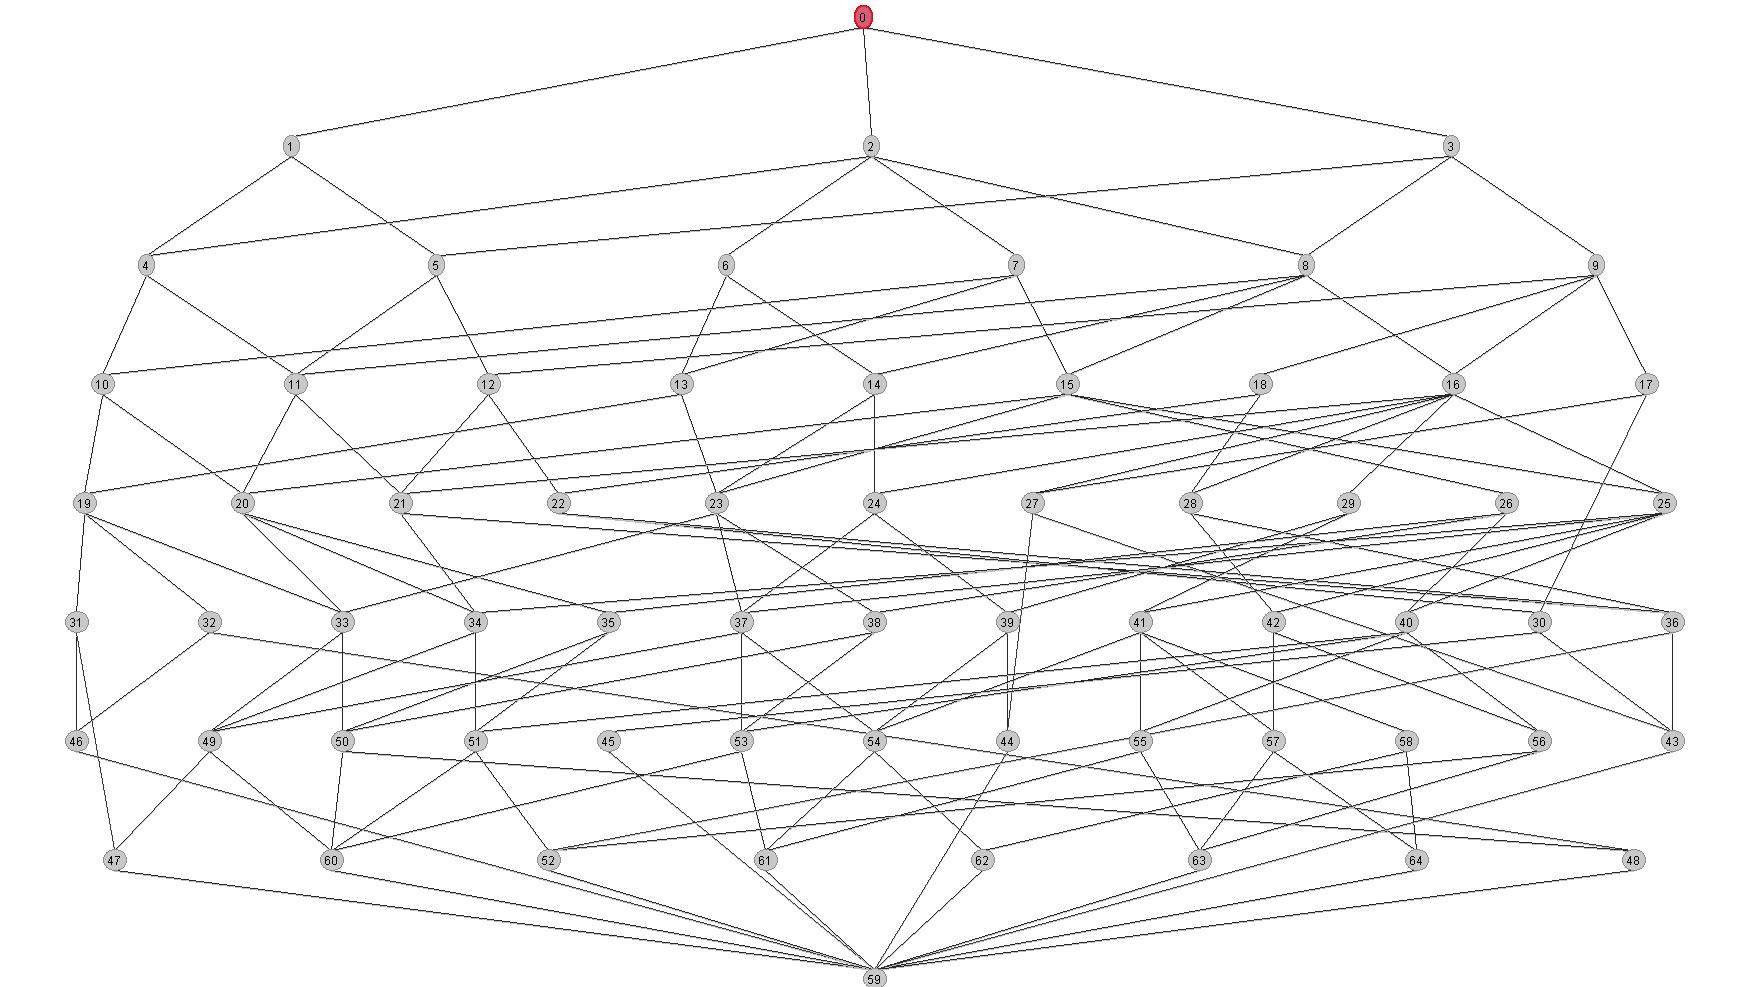
\includegraphics[width=0.7\textwidth]{treillis.png}
    \caption{Treillis de Galois de notre tableau}
    \label{fig:treillis} 
\end{figure}
\\
Dans un treillis de Galois, les nœuds situés aux extrémités correspondent soit à l’ensemble de tous les individus, soit à l’ensemble de toutes les caractéristiques. Ces nœuds étant trop généraux ou trop spécifiques, leur analyse n’est pas nécessaire. Nous concentrerons notre attention sur les nœuds possédant le plus grand nombre de connexions, car ils semblent jouer un rôle central en reliant plusieurs classes.
\\\\
\noindent $\bullet$ \underline{Nœud 16} : Ce nœud regroupe les documentaires (DA, DN, DS), les films (FC, FF, FD, FH, FP), les séries (SH, SP) ainsi que les clips chansons (CC). Ces individus partagent les caractéristiques suivantes : leur public cible est constitué d’adolescents ou d’adultes, leur objectif principal est la distraction, et ils sont réalisés en images réelles.
Ce nœud est significatif, car il relie une large gamme de types de médias (films, séries, documentaires, clips), montrant ainsi une diversité importante d'individus tout en restant centré sur des caractéristiques communes bien définies. Ce noeud représente les médias de divertissement en images réelles.
\\\\
\noindent $\bullet$ \underline{Nœud 25} : Ce nœud regroupe des contenus médiatiques (films, séries, clips) visant à divertir un public d'adolescents et d'adultes. Leur objectif est de fournir de l’évasion et de la distraction, sans intention éducative, tout en utilisant des images réelles pour offrir une expérience immersive et réaliste.
Il représente donc un espace de loisirs visuels. Ce nœud relie des contenus variés mais homogènes dans leur fonction sociale : divertir sans instruire.
\end{document}